\chapter{Support, Readability, and the Fallback}

The chapter develops a vocabulary the rest of the manual has used
implicitly: what does it mean to "support" a source. The vocabulary
matters because every product decision sits on top of it. A source
that is supported is one the product makes a correctness claim on; a
source that is merely readable is not. The two are easy to confuse.

\section{Four Properties, In Order}

\textbf{Observation.} Four properties characterise a source's
relationship to the parser. The order matters; each builds on the
last.

\begin{description}
  \item[Readable.] Raw bytes can be opened and sampled. A device file
    exists and \texttt{read()} returns data.
  \item[Parsable.] Checkpoint and root discovery succeed; raw
    traversal runs without aborting.
  \item[Validatable.] The parser's output can be compared to a named
    oracle for the requested mode. A namespace can be diffed
    against a POSIX traversal; a logical size against
    \texttt{st\_size}.
  \item[Supported.] The source is in the product allowlist for the
    requested mode. Validation has been performed; results were
    correct; the source class belongs in production.
\end{description}

The first three are technical. The fourth is editorial: it is the
project's decision about which sources are stable enough to make a
correctness claim on. A source can be readable and parsable and
validatable in one moment and not be supported because the moment is
not durable.

\section{Readable Is Not Supported}

The common confusion is between readability and support. A mounted
live volume is readable. It may, on a still moment, be parsable. It
may, against a momentary POSIX snapshot, even be validatable. It is
not supported, because the validation cannot be stable: the next
moment moves the visible checkpoint, the next POSIX snapshot
disagrees with the parser snapshot, and the user has no way to tell
which row is from which moment.

The right rule: support a source class only when the validation
recipe is reproducible. If the validation works once and then is
not reproducible because the source state has moved, the source
class is not supported even though one validation passed.

\section{The Current Allowlist}

The raw-mode allowlist is intentionally short.

\begin{itemize}
  \item Detached, unencrypted, image-backed APFS containers. The
    \texttt{.dmg} layer fixes the visible state at detach time.
  \item Caller-supplied raw APFS container devices under
    \texttt{/dev/disk*} or \texttt{/dev/rdisk*} where the caller
    has committed that the checkpoint will not advance.
  \item Explicitly stable APFS sources --- a tightly controlled lab
    volume where the operator pins the state.
\end{itemize}

What is not on the list: live mounted startup disks, FileVault
volumes the user is using, multi-device or Fusion containers,
sealed system volumes, snapshots opened through the operating
system's snapshot framework, and any container whose
\texttt{omap\_phys.flags} indicate an encryption operation in
flight.

The allowlist will grow only after a paired oracle and a new probe
clear the corresponding entry in the support matrix.

\section{EX-28 Live-Volume Raw Mode (Hypothesis C: Blocked by the Kernel)}
\label{sec:ex28-live-raw}

A live mounted volume's \texttt{/dev/diskNsM} device node is not on
the allowlist above. It cannot be: a live mounted volume is
exactly the case the source-gate refuses, because the volume
metadata advances during the scan window and SR-014 checkpoint
selection has no way to pin the visible state.

EX-28 asks the narrower question: \emph{if a user with root
privileges hands the existing raw parser a \texttt{/dev/diskNsM}
of a live volume, does the parser produce a self-consistent
shape, and does that shape agree with what the fallback walker
emits from the same mount point in the same scan window?}

The harness lands as a Rust integration test in
\texttt{crates/apfs-fastindex/tests/ex28\_live\_parity.rs},
gated on the environment variables
\texttt{APFS\_FASTINDEX\_EX28\_LIVE\_DEVICE} and
\texttt{APFS\_FASTINDEX\_EX28\_MOUNT\_POINT}. Without those, the
test is a clean no-op and \texttt{cargo test --release} skips it.
With them set and the test run as root, the harness:

\begin{enumerate}
  \item Tries three successive raw scans of the device. Each
    must publish a \texttt{selected\_checkpoint} (no SR-014
    fail-closure under live concurrent writes), with pairwise
    symmetric difference of their \texttt{NamespaceEntry} sets
    $\leq 200$ paths.
  \item Runs one fallback-walker scan of the mount point and
    compares it against the raw scan; symmetric difference must
    be $\leq 1000$ paths to absorb the
    raw-can-read-paths-the-fallback-cannot asymmetry (TCC, sealed
    system volume reads).
\end{enumerate}

The comparator behind both checks is
\texttt{apfs\_fastindex::parity::compare\_namespace\_shapes},
which returns a structured \texttt{ShapeDiff} with
\texttt{only\_in\_left}, \texttt{only\_in\_right}, and per-field
\texttt{mismatches}. It is exposed as a public crate surface so
any future tooling can use it.

\textbf{Observation (2026-05-20).} The first privileged run on
the project owner's Apple silicon host returned the harshest of
the planned fallbacks: macOS refused to even open
\texttt{/dev/disk3s1} for raw reads, returning \texttt{EPERM}
(errno 1, ``Operation not permitted'') on the first
\texttt{read(2)} of the device's block zero, despite the
process running as root. The harness classifies this as
\texttt{LiveScanOutcome::BlockedByKernel} and records the
\texttt{live\_raw\_blocked\_by\_kernel} verdict. The kernel's
storage-system security policy refuses raw block access to the
live boot data partition independently of POSIX file
permissions; SIP and the sealed-system-volume seal both
contribute. Neither the successive-scan stability nor the
raw-vs-fallback parity assertions could be evaluated because the
raw backend never opened.

\textbf{Product implication.} The "Scan as administrator…" menu
item the original EX-28 plan anticipated does not graduate to
raw mode on a stock Apple silicon macOS host. The
privileged-subprocess shape still serves a purpose --- unlocking
TCC-restricted user-data paths the fallback walker hits
\texttt{EACCES} on --- but it stays on the fallback walker even
under root. The raw fast path is unchanged in its original scope:
detached \texttt{.dmg} images, caller-pinned raw devices on a
quiesced volume. EX-28's contribution to the codebase is the
reusable shape-parity comparator
(\texttt{apfs\_fastindex::parity}) and the env-gated integration
harness that future hosts (or future macOS versions with
different security policies) can rerun without code changes.

The live-disk row of the support matrix therefore reads:
\emph{not supported on stock macOS; raw read returns
\texttt{EPERM} under \texttt{sudo}; the fallback walker remains
authoritative for live volumes, including the
privileged-subprocess invocation that unlocks TCC-restricted
user-data paths.}

\section{EX-29 Local-Snapshot Enumeration (No User Snapshots
on This Host)}
\label{sec:ex29-snapshots}

The product surfaces local snapshots as a row in the status bar
because their bytes are part of \texttt{df}'s ``used'' total and
the volume's Finder-reported capacity, but the scanner walks
only the live volume's fs-tree. Without a snapshot row, those
bytes look ``missing'' on a user's mental model.

EX-29's deliverable is the enumeration: a count of user-visible
local snapshots, with names. Reclaimable bytes are explicitly
out of scope on stock Apple silicon: there is no public
read-only oracle for per-snapshot reclaimable bytes
(\texttt{tmutil thinlocalsnapshots} reports the number, but it
deletes the snapshot in the process), and EX-28's verdict
(\texttt{live\_raw\_blocked\_by\_kernel}) ruled out the raw
extent-set diff path.

Enumeration is unprivileged. The crate's
\texttt{snapshots} module calls \texttt{tmutil
listlocalsnapshots <mount>} and \texttt{diskutil apfs
listSnapshots <mount>}, parses each output, and classifies the
result. SR-020's sealed-system filter excludes snapshots whose
name matches \texttt{com.apple.os.update-*} (the read-only
system volume's boot snapshot, which the user can't delete and
whose bytes aren't user-visible).

\textbf{Observation (2026-05-20).} The project owner's host
has zero user-visible TM local snapshots and one sealed-system
OS-update snapshot on \texttt{disk3s1s1}. The classifier
returned \texttt{NoUserSnapshots\{sealed\_system\_excluded\_count
= 1\}}. EX-23 found the same shape in 2026-05-16; on a
single-user development host without Time Machine configured
this is the expected steady state.

The integration harness in
\texttt{crates/apfs-fastindex/tests/ex29\_snapshot\_enumeration.rs}
mirrors EX-28's pattern. An unconditional unprivileged test runs
the classifier; a gated test exercises a raw extent diff between
a mounted snapshot's device node and the live volume, using the
existing \texttt{parity::compare\_namespace\_shapes} comparator.
The gated test reuses EX-28's \texttt{LiveScanOutcome}
classifier, so an \texttt{EPERM} on the snapshot device is
recorded as ``EX-28 Hypothesis C reproduces on the snapshot
device'' rather than failing the test.

The live-snapshot row of the support matrix therefore reads:
\emph{enumeration validated; reclaimable bytes unclaimed (no
read-only oracle; raw extent diff blocked by EX-28 Hypothesis C
on Apple silicon under SIP).}

\section{Fail-Closed Triggers}

A source that does not satisfy the allowlist must fail closed before
emitting rows. The categorical triggers, with the chapter that
develops each:

\begin{description}
  \item Ambiguous or malformed checkpoint state (chapter~3).
  \item Non-contiguous checkpoint descriptor layout (chapter~3).
  \item Unsupported incompatible feature bits in the container or
    volume (chapter~3, chapter~5).
  \item OMAP-open or OMAP-lookup encryption flags (chapter~4).
  \item Unknown bits in any \texttt{flags} field the parser inspects
    (chapter~4, chapter~7).
  \item Encryption keys or hardware-backed key requirements the
    parser cannot reach (chapter~4).
  \item Fusion or multi-device storage requirements (chapter~3).
  \item Requested merged-root or boot-root semantics (chapter~13).
  \item Snapshot or sealed-volume semantics outside the target mode
    (chapter~13).
  \item No validated corpus for the source class.
\end{description}

Each trigger is a typed error with a substring naming the rule. The
caller dispatches on the error rather than retrying.

\section{The Fallback}

When the parser refuses a source, the product is not stuck. The
fallback path emits the same shape of output through supported
operating-system APIs.

\textbf{Observation.} A POSIX-traversal fallback in both Python
(\texttt{fallback\_traversal.py}) and Rust (\texttt{fallback.rs})
emits \texttt{NamespaceEntry} and \texttt{DirectoryAggregate} rows
that, on the proof fixture, match the raw-mode output of the same
volume exactly. Same entry count, same paths, same
\texttt{entry\_kind}, same \texttt{logical\_size}, same
\texttt{symlink\_target}, same per-directory aggregates.

The fallback walker uses \texttt{os.walk} plus \texttt{os.lstat} plus
\texttt{os.readlink} in the Python version, and the equivalent
\texttt{read\_dir} plus \texttt{symlink\_metadata} plus
\texttt{read\_link} in the Rust version. Both paths apply the SR-017
precedence rule at the trivial step: \texttt{st\_size} for regular
files, \texttt{readlink} byte length for symlinks. Both apply the
unique-inode aggregate policy from chapter~8.

Two consequences follow.

\paragraph{The contract is mode-independent.} The product emits the
same shape of output regardless of which backend produced it. The
caller does not have to know whether the row came from a raw FS-tree
walk or a POSIX traversal; the field set and the semantic mode are
identical.

\paragraph{The slow path is not slow.} Chapter~12 shows that the
parallel fallback (four workers by default) sustains roughly 313
thousand entries per second on warm directory trees on Apple
silicon --- 2.47$\times$ the post-micro-optimisation single-threaded
throughput and 1.82$\times$ the pre-perf baseline. On a cold
whole-machine scan the bottleneck is the disk, not the parser. The
fallback is fast enough to be the default for sources outside the
raw allowlist, not a degraded mode.

\section{Resilience In The Fallback}

A whole-machine scan as a normal user encounters paths that the
user does not have permission to read: sandboxed application data,
sealed-system directories, daemon-owned caches. The fallback walker
must continue across these without aborting and without producing
silently incomplete totals.

\textbf{Observation.} Per-entry \texttt{EACCES}, \texttt{EPERM}, and
\texttt{ENOENT} are recorded in \texttt{parser\_output.walk\_skips}
with a reason; the walk continues. The same log carries the
\texttt{firmlink\_overlay\_source} and \texttt{duplicate\_dir\_inode}
skip kinds introduced by the dedup pass below. A normal-user
\texttt{/} scan on the host the project tested completes with
roughly five hundred recorded skips (the exact count varies with
the host's app sandbox profile and the firmlink set) and reports
them in the output document. The caller can render the skip list
as a diagnostic without it affecting the row stream.

The walker also skips top-level system directories that exist only as
APFS-internal artefacts on the boot disk
(\texttt{.fseventsd}, the system snapshot mountpoints) by name,
rather than letting the operating system raise an error on them.
That skip is documented in the source so it can be revisited as
support broadens.

\section{Parallel Fallback}

\textbf{Observation.} The fallback walker accepts a
\texttt{--threads N} flag. The default is
\texttt{min(hw.physicalcpu, 4)}; the lower bound is 1, the upper
bound clamped to 4. Per-worker \texttt{BulkReader} owns its own
64~KiB \texttt{getattrlistbulk} buffer; a shared work queue
distributes directories; per-worker entry vectors are
concatenated and re-sorted on the main thread.

The default's ceiling at 4 is not arbitrary. The single APFS
container holds a B-tree contention point that pre-Mojave was
described as a global mutex (Szorc 2018) and that the Apple
Developer Forums position (Apple DTS, 2025) describes as having
been largely addressed in macOS~10.14 while leaving a residual
per-container cost. Empirical measurement on Apple silicon
(EX-25, chapter~12) shows the throughput envelope peaking at
$T = 4$ with 2.47$\times$ speedup over single-threaded, then
\emph{regressing} at $T = 8$ and falling further at $T = 14$. At
$T = 8$ the total system CPU is $4\times$ the $T = 1$ value while
the throughput is only $1.94\times$; at $T = 14$ system CPU is
$9.3\times$ for $1.38\times$ throughput --- the kernel pays
super-linearly more work to deliver sub-linearly more answers.
The 4-thread ceiling stays clear of that regime by construction.

The parallel walker preserves the serial walker's contract by
shape, asserted by a synthetic-tree regression test
(\texttt{parallel\_walker\_matches\_serial\_shape}): identical
entries, aggregates, and skip lists; the only difference is the
order in which directories are visited, which the final sort
normalises.

Live progress events flow through a dedicated sampling thread
inside the parallel scheduler at a 250~ms cadence (matching the
serial path), so the CLI's \texttt{-{}-progress} stream and any
user-space consumer of it can tick smoothly even on a
whole-machine scan that is otherwise silent for tens of seconds.
The in-process FFI consumed by the native shell of chapter~13
exposes the same stream through
\texttt{apfs\_scan\_directory\_with\_progress}, which takes a
\texttt{(*const c\_void, ApfsProgressEvent*)} callback the
sampling thread invokes from the library side; the SwiftUI shell
hands in a closure that updates an \texttt{@Published}
\texttt{ProgressSnapshot} on the main actor and the toolbar's
determinate progress bar follows it. The serial-vs-parallel
cadence and event payload are identical across the CLI and the
FFI; one source of truth, two delivery surfaces.

\begin{figure}[h]
\centering
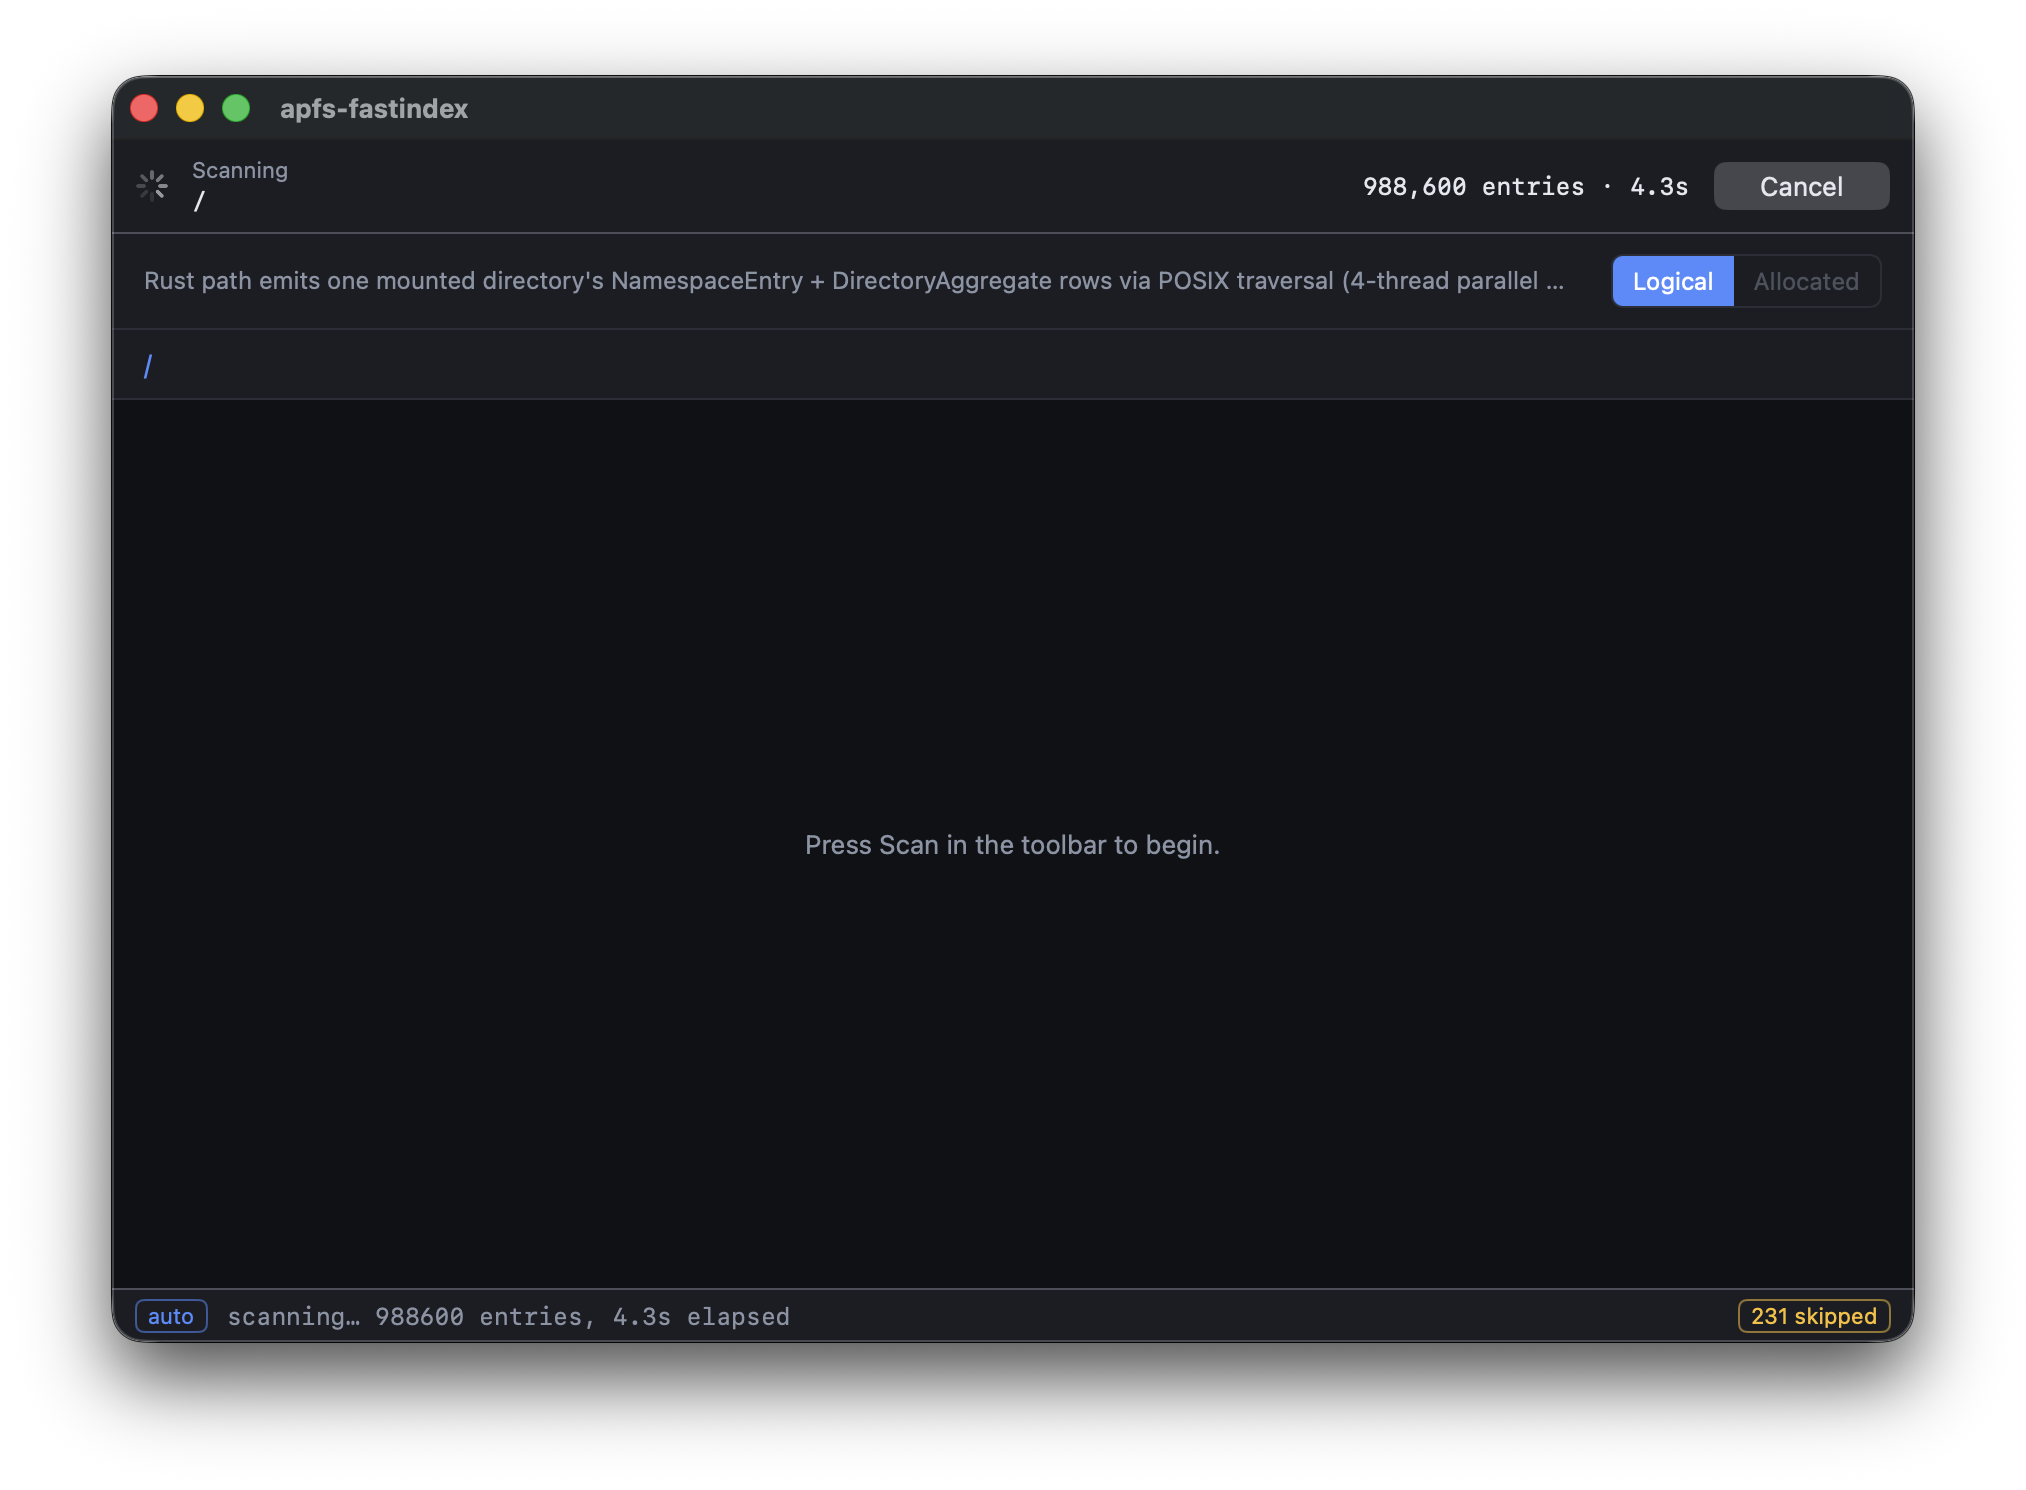
\includegraphics[width=\linewidth]{figures/app-progress.png}
\caption{A whole-machine \texttt{/} scan mid-flight in the
pre-native build that consumed \texttt{-{}-progress} stderr
events. The stopwatch and entry counter come from the parallel
walker's progress thread; 231 paths have been recorded as
skipped at this point in the walk (sandboxed application data,
sealed-system locations). The Cancel control terminates the
worker pool cleanly. The same event stream now also flows into
the native shell through
\texttt{apfs\_scan\_directory\_with\_progress}, which carries
the cumulative logical-bytes count as well so the SwiftUI
shell's progress bar is determinate rather than spin-wait
indeterminate.}
\end{figure}

\section{Firmlink Overlay Dedup}

\textbf{Observation.} On macOS the user-visible startup root is a
join of the System volume and the Data volume. Specific paths ---
\texttt{/Users}, \texttt{/Applications}, \texttt{/Library},
\texttt{/private}, \texttt{/usr/local}, and a few others --- are
exposed both at their canonical location \emph{and} at
\texttt{/System/Volumes/Data/<source>} via firmlinks. The same
underlying inode is visible through two paths. A naive recursive
walker descends both and double-counts everything inside the
overlay.

The fallback walker, when the root is \texttt{/}, reads
\texttt{/usr/share/firmlinks} at scan-start and builds a
\texttt{HashSet} of the \texttt{/System/Volumes/Data/<source>}
overlay paths. A descent into any such path is refused with a
\texttt{firmlink\_overlay\_source} skip; the canonical path
remains the one that contributes to the namespace and aggregates.

A second layer of safety, a per-scan
\texttt{Mutex<HashSet<(dev, ino)>>}, catches any directory
inode reached through a path the firmlink overlay set did not
cover. A second observation of the same inode through a different
path is recorded as a \texttt{duplicate\_dir\_inode} skip and the
walker does not recurse.

The effect on whole-machine scans is large. Before the dedup, a
\texttt{/} scan on the test host reported 5,250,000 entries;
after, 3,060,000 entries with seventeen
\texttt{firmlink\_overlay\_source} skips (one per existing
firmlink target) and zero \texttt{duplicate\_dir\_inode} skips
(the overlay layer caught everything). The forty-two per cent
that disappeared were not real files: they were the same files
counted twice through two paths.

\section{Auto-Dispatch}

The CLI binary \texttt{apfs-fastindex-scan} picks the backend
automatically based on the source path's shape.

\begin{itemize}
  \item A \texttt{.dmg} path or a \texttt{/dev/disk*} /
    \texttt{/dev/rdisk*} device path is dispatched to raw mode.
  \item A directory path is dispatched to fallback mode.
  \item The caller can override with \texttt{--mode raw},
    \texttt{--mode fallback}, or \texttt{--mode auto}.
\end{itemize}

The auto-dispatch is what makes the support boundary usable as a
product surface. The user does not have to remember which sources
are in the allowlist; the binary handles the dispatch and tells the
caller, through the \texttt{correctness\_claim} and
\texttt{not\_claimed} fields, which mode actually ran.

\section{Why The Boundary Is Permanent}

The boundary between raw and fallback is not provisional. As the
allowlist grows (chapter~13 tracks the open candidates), each new
source class gets its own line in the support matrix: its own
allowlist row, its own oracle, its own probe. The boundary moves
only when there is evidence to move it.

This means the manual will keep growing chapters of this shape:
``\emph{here is the source class, here is the oracle, here is the
probe, here is the result, here is the support claim}.'' The work
finishes only when every source class an APFS reader is willing to
claim has its own line in the matrix.

The unsexy form of the work is the price of having a fast indexer
that is also correct.
